
The general equation of a circle is given by
\begin{align}
  \vec{x}^T\vec{x}-2\vec{c}^T\vec{x}+f = 0 \label{eq:solutions/4/1/1/c/eq2}
\end{align}
where $\vec{c}$ is the centre of the circle and r = $\sqrt{\norm{\vec{c}}^2-f}$ is the radius of the circle.
Dividing \eqref{eq:solutions/4/1/1/c/eq1} by 2 and rearranging terms \eqref{eq:solutions/4/1/1/c/eq1} can be rewritten as 
\begin{align}
  \vec{x}^T\vec{x}-2\myvec{-4\\1}^T\vec{x}+\frac{33}{2} = 0 \label{eq:solutions/4/1/1/c/eq3}
\end{align}
Comparing \eqref{eq:solutions/4/1/1/c/eq2} and \eqref{eq:solutions/4/1/1/c/eq3} we get
\begin{align}
  &\vec{c} = \myvec{-4\\1}\\
  &f = \frac{33}{2}
\end{align}
Then centre of the circle \eqref{eq:solutions/4/1/1/c/eq1} is $\vec{c}$ = $\myvec{-4\\1}$ and radius
\begin{align}
  r &= \sqrt{\norm{\vec{c}}^2-f}\\
  &= \sqrt{(-4)^2+1^2-\frac{33}{2}}\\
  &= \sqrt{\frac{1}{2}}\\
  &= 0.7071
\end{align}
  \begin{figure}[!ht]
	\centering
	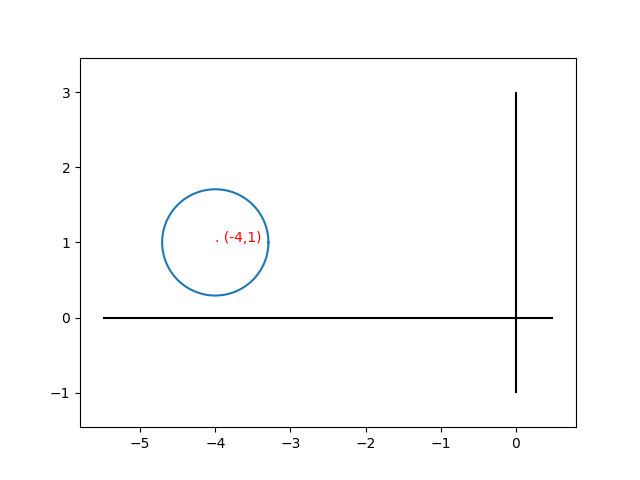
\includegraphics[width=\columnwidth]{./solutions/4/1/1/c/circle.png}
	\caption{Graph of $2x^2+2y^2+16x-4y+33=0$}
	\label{eq:solutions/4/1/1/c/myfig}
\end{figure}
